\documentclass{article}

\usepackage[top=1in,left=1.5in,right=1.5in,bottom=1.5in]{geometry}

\usepackage{subcaption}

\usepackage{booktabs}

\usepackage{graphicx}
\let\rfb\reflectbox
\graphicspath{ {images} }
 
\usepackage{cancel}

\usepackage{mathtools}

\usepackage{nicefrac}
\newcommand{\flippedfrac}[2]{\rfb{\nicefrac{\rfb{#2}}{\rfb{#1}}}}



\usepackage{amsthm}
\renewcommand{\qedsymbol}{$\blacksquare$}
\usepackage{amssymb}
\usepackage{amsmath}
\newcommand\numberthis{\addtocounter{equation}{1}\tag{\theequation}}
\DeclareMathOperator*{\argmax}{arg\,max}
\DeclareMathOperator*{\argmin}{arg\,min}

\usepackage{hyperref}
\hypersetup{
    colorlinks = true,
}


\usepackage{titling}
\title{Exercise Set 3 - Reinforcement Learning}
\newcommand{\subtitle}[1]{%
  \posttitle{%
    \par\end{center}
    \begin{center}\large#1\end{center}
    \vskip0.5em}%
}
\makeatother
\subtitle{Advanced TD methods and approximation}
\author{Giulio Starace - 13010840}
\date{\today}

\begin{document}
\maketitle
\section*{Homework: Coding Assignment - Temporal Difference Learning}
\begin{enumerate}
	\item Coding answers have been submitted on codegra under the group ``stalwart cocky sawly".
	\item As can be seen in Fig. \ref{fig:sarsa_v_qlearning}, Q-learning achieves higher average
	      return for the particular environment considered. This is the opposite of Example 6.6 in the
	      book where SARSA achieves higher average return. This is due to the difference between
	      environments. In Example 6.6, the environment contains a penalty cliff adjacent to the
	      optimal path, causing optimally acting agents (converged q-learners) to risk incurring high
	      penalties. This is unlike the environment considered in this homework, where the optimal
	      path is in a sense ``risk-free'', allowing Q-learning to outperform SARSA.
	      \begin{figure}[ht]
		      \centering
		      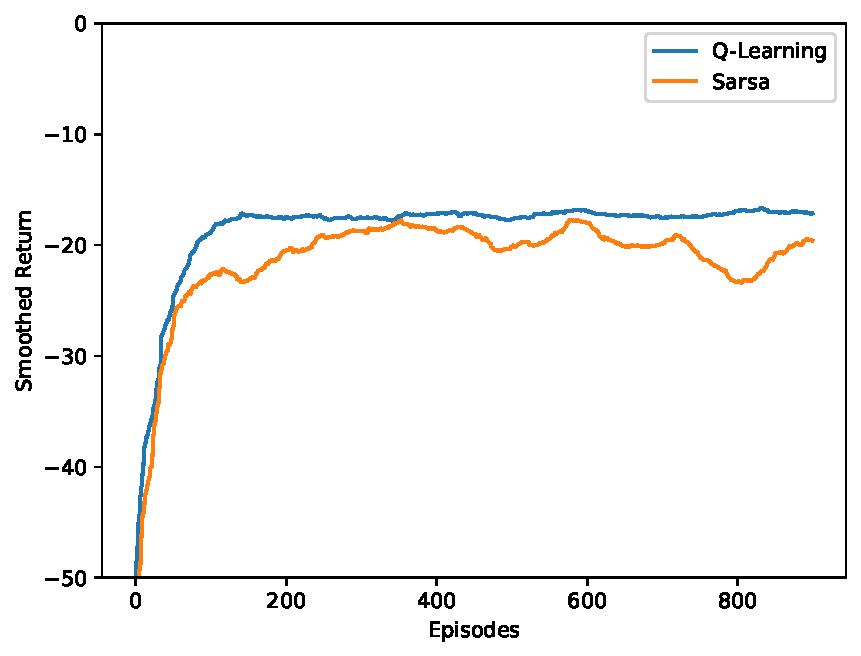
\includegraphics[width=\textwidth]{sarsa_v_qlearning}
		      \caption{SARSA vs Q-learning average return over number of episodes for the Windy
			      Gridworld environment.}
		      \label{fig:sarsa_v_qlearning}
	      \end{figure}
\end{enumerate}

\section*{Homework: Maximization Bias}
\begin{enumerate}
	\item For the sake of clarity, we label the four outgoing actions from $B$ as $a_1$, $a_2$, $a_3$
	      and $a_4$, from left to right, and say they belong to the action set $A$. For expected
	      SARSA, we use the expected SARSA update rule to determine the state-action values:
	      \begin{align*}
		      Q(S_t, A_t) & \leftarrow Q(S_t, A_t) + \alpha \left[ R_{t+1} + \gamma \mathbb{E}_\pi
		      \left[Q(S_{t+1}, A_{t+1})|S_{t+1}\right]  - Q(S_t, A_t) \right]                            \\
		                  & = Q(S_t, A_t) + \alpha \left[ R_{t+1} + \gamma \sum_{a \in A} \pi(a|S_{t+1})
			      Q(S_{t+1}, a) - Q(S_t, A_t) \right]. \numberthis \label{eq:expected_sarsa_update}
	      \end{align*}
	      Because all actions from $B$ lead to a terminal state, we have that $Q(S_{t+1}, a) = 0$ for
	      all $a \in A$ when $S_t = B$.

	      For $a_1$, on the first relevant sampled episode we have $R_{t+1} = 0$ giving:
	      \begin{align*}
		      Q(B, a_1) & \leftarrow  0.7 + 0.2 \left[ 0 +\cancelto{0}{1 \times 4(0.25 \times 0)}
		      - 0.7 \right]                                                                       \\
		                & = 0.7 + 0.2 \left[- 0.7 \right]                                         \\
		                & = 0.56.\numberthis                                                      \\
	      \end{align*}
	      And on the next relevant sampled episode we get the same reward, giving:
	      \begin{align*}
		      Q(B, a_1) & \leftarrow 0.56 + 0.2 \left[0 + \cancelto{0}{1 \times 4(0.25 \times 0)} - 0.56
		      \right]                                                                                    \\
		                & = 0.56 + 0.2 \left[- 0.56 \right]                                              \\
		                & = 0.448.\numberthis
	      \end{align*}
	      For $a_2$, on the first relevant sampled episode we have $R_{t+1} = 1$, giving:
	      \begin{align*}
		      Q(B, a_2) & \leftarrow 0.7 + 0.2 \left[ 1 + \cancelto{0}{1 \times 4(0.25 \times 0)} - 0.7
		      \right]                                                                                   \\
		                & = 0.7 + 0.2 \left[0.3 \right]                                                 \\
		                & = 0.76. \numberthis
	      \end{align*}
	      And on the next relevant sampled episode, we get the same reward, giving:
	      \begin{align*}
		      Q(B, a_2) & \leftarrow 0.76 + 0.2 \left[ 1 + \cancelto{0}{1 \times 4(0.25 \times 0)}
		      - 0.76 \right]                                                                       \\
		                & = 0.76 + 0.2 \left[0.24 \right]                                          \\
		                & = 0.808. \numberthis
	      \end{align*}
	      For $a_3$, on the first relevant sampled episode we have $R_{t+1} = 1$, which we know from
	      the first update to $a_2$ gives us
	      \begin{equation}
		      Q(B, a_3) \leftarrow 0.76.
	      \end{equation}
	      On the next relevant sampled episode, we have $R_{t+1} = 0$, giving:
	      \begin{align*}
		      Q(B, a_2) & \leftarrow 0.76 + 0.2 \left[ 0 + \cancelto{0}{1 \times 4(0.25 \times 0)}
		      - 0.76 \right]                                                                       \\
		                & = 0.76 + 0.2 \left[-0.76 \right]                                         \\
		                & = 0.608. \numberthis
	      \end{align*}
	      For $a_4$, on the first relevant sampled episode we have $R_{t+1} = 0$, which we know from
	      the first update to $a_1$ gives us
	      \begin{equation}
		      Q(B, a_4) \leftarrow 0.56.
	      \end{equation}
	      On the next relevant sampled episode, we have $R_{t+1} = 1$, giving:
	      \begin{align*}
		      Q(B, a_1) & \leftarrow 0.56 + 0.2 \left[1 + \cancelto{0}{1 \times 4(0.25 \times 0)} - 0.56
		      \right]                                                                                    \\
		                & = 0.56 + 0.2 \left[0.44 \right]                                                \\
		                & = 0.648.\numberthis
	      \end{align*}
	      For Q-learning, we use the Q-learning update rule to determine the state-action values:
	      \begin{equation}
		      Q(S_t, A_t) \leftarrow Q(S_t, A_t) + \alpha \left[ R_{t+1} + \gamma \max_{a \in A}
			      Q(S_{t+1}, a) - Q(S_t, A_t) \right].\label{eq:q_learning_update}
	      \end{equation}
	      Note once again that since when $S_t = B$, $S_{t+1}$ is always a terminal state, then like
	      before $Q(S_{t+1}, a) = 0$ for all $a \in A$. Therefore, in this case, equation
	      (\ref{eq:q_learning_update}) reduces like equation (\ref{eq:expected_sarsa_update}) to
	      \begin{equation}
		      Q(S_t, A_t) \leftarrow Q(S_t, A_t) + \alpha \left[ R_{t+1} - Q(S_t, A_t)
			      \right]. \label{eq:terminal_reduction}
	      \end{equation}
	      Therefore, all the state-action values in state $B$ are the same in Q-learning as for
	      expected SARSA. For a clearer summary, refer to Table \ref{tab:b_qvalues}.
	      \begin{table}[ht]
		      \centering
		      \caption{Expected SARSA and Q-learning state-action pair values for the four available
			      actions at state $B$ after sampling two episodes per action.}
		      \label{tab:b_qvalues}
		      \begin{tabular}{@{}rcccc@{}}
			      \toprule
			                              & $Q(B, a_1)$ & $Q(B, a_2)$ & $Q(B, a_3)$ & $Q(B, a_4)$ \\ \midrule
			      \textbf{expected SARSA} & 0.448       & 0.808       & 0.608       & 0.648       \\
			      \textbf{Q-learning}     & 0.448       & 0.808       & 0.608       & 0.648       \\ \bottomrule
		      \end{tabular}
	      \end{table}
	\item To determine what the new $Q(A, L)$ value is when executing $L$ in $A$ after the 10
	      episodes, assuming that $Q(A, L)$ is still at 0.7, we use the same update rules as stated
	      before, i.e. equation (\ref{eq:expected_sarsa_update}) for expected SARSA and equation
	      (\ref{eq:q_learning_update}) for Q-learning. Since taking $L$ at $A$ leads to a terminal
	      state, equations (\ref{eq:expected_sarsa_update}) and (\ref{eq:q_learning_update}) once
	      again reduce to equation (\ref{eq:terminal_reduction}). For both expected SARSA and
	      Q-learning we therefore have:
	      \begin{align*}
		      Q(A, L) & \leftarrow 0.7 + 0.2 \left[ 0.7 - 0.7 \right] \\
		              & = 0.7 + 0.2 \left[ 0 \right]                  \\
		              & = 0.7. \numberthis
	      \end{align*}
	      We apply the same process to determine what the new $Q(A, R)$ value is when executing $R$ in
	      $A$ after the 10 episodes, assuming that $Q(A, R)$ is still at 0.7. However, the reduction
	      to equation (\ref{eq:terminal_reduction}) is not possible in this case, since $R$ from $A$
	      does not transition to a terminal state. With expected SARSA we have
	      \begin{align*}
		      Q(A, R) & \leftarrow 0.7 + 0.2 \left[ 0 + 0.25\left(0.448 + 0.808 + 0.608 + 0.648\right)
		      - 0.7\right]                                                                             \\
		              & = 0.6856. \numberthis
	      \end{align*}
	      With Q-learning, we have
	      \begin{align*}
		      Q(A, R) & \leftarrow 0.7 + 0.2 \left[ 0 + 0.808 - 0.7 \right] \\
		              & = 0.7216. \numberthis
	      \end{align*}
	      For a clearer summary, please refer to Table \ref{tab:a_lr_qvalues}.
	      \begin{table}[ht]
		      \centering
		      \caption{Expected SARSA and Q-learning state-action pair values at $A$ when executing $R$
			      and $L$ from $A$ after the 10 sampled episodes.}
		      \label{tab:a_lr_qvalues}
		      \begin{tabular}{@{}ccc@{}}
			      \toprule
			                & \textbf{Expected SARSA} & \textbf{Q-learning} \\ \midrule
			      $Q(A, L)$ & 0.7                     & 0.7                 \\
			      $Q(A, R)$ & 0.6856                  & 0.7216              \\ \bottomrule
		      \end{tabular}
	      \end{table}
	\item Assuming convergence to optimality for both Q-learning and Expected SARSA, we can obtain the
	      true state-action values by utilising the Bellman optimality equation:
	      \begin{equation}
		      q_*(s, a) = \sum_{s', r} p(s', r \mid s, a) \left[ r + \gamma \max_{a'} q_*(s', a') \right].
	      \end{equation}
	      The results of applying this equation to our MDP are summarised in Table
	      \ref{tab:true_qvalues}.
	      \begin{table}[ht]
		      \centering
		      \caption{True state-action values after Expected SARSA and Q-learning convergence.}
		      \label{tab:true_qvalues}
		      \begin{tabular}{@{}cccccc@{}}
			      \toprule
			      \textbf{$Q_*(A, L)$} & \textbf{$Q_*(A, R)$} & $Q_*(B, a_1)$ & $Q_*(B, a_2)$ & $Q_*(B, a_3)$ & $Q_*(B, a_4)$ \\ \midrule
			      0.7                  & 0.5                  & 0.5           & 0.5           & 0.5           & 0.5           \\ \bottomrule
		      \end{tabular}
	      \end{table}
	\item Maximization bias can be observed in all estimated state-action values reported in Tables
	      \ref{tab:b_qvalues} and \ref{tab:a_lr_qvalues}, except for $Q(A, L)$ and $Q(B, a_1)$. We
	      observe maximization bias here as the estimated values are higher than the true values
	      reported in Table \ref{tab:true_qvalues}, i.e. they are positively biased. Both Q-learning
	      and expected SARSA are affected by this bias, as both algorithms rely on a greedy (target)
	      policy which requires the use of a maximum operator. When coupled with stochastic
	      transitions and rewards, such as in our MDP from state $B$, this generally leads to
	      a positive bias in the estimated state-action values.
	\item Double Q-learning circumvents the issue of maximization bias in Q-learning by using two
	      independent estimates, $Q_1$ and $Q_2$, of the true value function $q$. This is unlike
	      vanilla Q-learning where we use a single estimate $Q$. The two estimates afford us the
	      possibility of using one estimate for determining the greedy action $A^* = \argmax_aQ_1(a)$
	      and the other for estimating its value $Q_2(A^*) = Q_2(\argmax_aQ_1(a))$. The latter estimate
	      is then unbiased: $\mathbb{E}\left[Q_2(A^*)\right] = q(A^*)$. We can then repeat the process
	      with $Q_1$ and $Q_2$ swapped to obtain another unbiased estimate. More specifically, in
	      double Q-learning for any given timestep $t$ we would, with probability 0.5, use the
	      following update rule:
	      \begin{equation}
		      Q_1(S_t, A_t) \leftarrow Q_1(A_t, A_t) + \alpha \left[ R_t + \gamma Q_2(S_{t+1},
			      \argmax_{a}Q_1(S_{t+1}, a)) - Q_1(S_t, A_t) \right],
	      \end{equation}
	      and flip the roles of $Q_1$ and $Q_2$ otherwise. For a more concrete example, consider the
	      estimate of $q(A, R)$, whose true value is 0.7 but we have estimated to be 0.7216 in
	      vanilla Q-learning as shown in Table \ref{tab:a_lr_qvalues}. Under Double Q-learning, still
	      assuming an initialization of 0.7, our estimate would now look like:
	      \begin{align*}
		      Q_1(a, r) & \leftarrow 0.7 + 0.2 \left[ 0 + Q_2(b, a_2) - 0.7\right] \\
		                & = 0.7 + 0.2 \left[ 0.7 - 0.7\right]                      \\
		                & = 0.7. \numberthis
	      \end{align*}
	      We can repeat this process with $Q_1$ and $Q_2$ swapped to obtain another unbiased estimate:
	      \begin{align*}
		      Q_2(A, R) & \leftarrow 0.7 + 0.2 \left[ 0 + Q_1(B, a_2) - 0.7\right] \\
		                & = 0.7 + 0.2 \left[ 0.7 - 0.7\right]                      \\
		                & = 0.7. \numberthis
	      \end{align*}
	      We see that our estimate has now been reduced from 0.7216 to 0.7, the true value, thus
	      circumventing the maximization bias issue.
\end{enumerate}

\section*{Homework: Gradient Descent Methods}
\begin{enumerate}
	\item The true value of a state $v_\pi(S_t)$ is defined to be the expected return at that state,
	      i.e.
	      \begin{equation}
		      v_\pi(S_t) = \mathbb{E}\left[ G_t \mid S_t = s \right].
	      \end{equation}
	      Since the Monte Carlo target \textit{is} the return $G_t$, estimated using direct samples of
	      the true value, it has the same expected value as $v_\pi(S_t)$ and is therefore an unbiased
	      estimate of the true value of a state by definition.
	\item The temporal difference (TD) error, $\delta_t$ is given by
	      \begin{equation}
		      \delta_t ~\dot{=}~ R_{t+1} + \gamma V(S_{t+1}) - V(S_t).\label{eq:td_err}
	      \end{equation}
	      A weight update that minimizes the mean squared temporal difference error
	      $\overline{\delta_t}$ can be derived by considering the definition of mean square
	      \textit{value} error $\overline{\text{VE}}$:
	      \begin{equation}
		      \overline{\text{VE}} ~ \dot{=} ~ \sum_{s \in \mathcal{S}} \mu(s) \left[v_\pi(s)
			      - \hat{v}(s, \mathbf{w})\right]^2,
	      \end{equation}
	      where $\hat{v}$ is our approximation and $v_\pi$ is the true value. Here we have the squared
	      error term in the brackets, weighted by ``how much we care about it'', $\mu(s)$ in a sum. We
	      can replace the error term in the brackets with the TD error given in equation
	      (\ref{eq:td_err}), obtaining
	      \begin{equation}
		      \overline{\delta_t} = \sum_{s_t, s_{t+1} \in \mathcal{S}} \mu(s) \left[R_{t+1} + \gamma
			      \hat{v}(s_{t+1}, \mathbf{w}) - \hat{v}(s_t, \mathbf{w}))\right]^2,
	      \end{equation}
	      where we are now summing over all possible state transitions $(s_t, s_{t+1})$.  We can then
	      find the weight update rule that minimizes the mean squared TD error by taking the gradient
	      with respect to $\mathbf{w}$:
	      \begin{align*}
		      \mathbf{w}_{t+1} & \leftarrow \mathbf{w}_t - \frac{1}{2} \alpha \nabla\left[R_{t+1}
		      + \gamma \hat{v}(s_{t+1}, \mathbf{w}) - \hat{v}(s_t, \mathbf{w}))\right]^2          \\
		                       & = \mathbf{w}_t + \alpha \left[R_{t+1} + \gamma \hat{v}(s_{t+1},
		      \mathbf{w}) - \hat{v}(s_t, \mathbf{w}))\right] \nabla \hat{v}(s_t, \mathbf{w})      \\
		                       & = \mathbf{w}_t + \alpha \delta_t \nabla \hat{v}(s_t,
		      \mathbf{w}). \numberthis
	      \end{align*}
	      This is precisely the same result as Semi-Gradient TD(0). We note that semi-gradient methods no
	      longer make use of information from the true target value, $v_\pi$, instead only accounting
	      for changes on the estimates. In this sense, only a portion of the true gradient is
	      considered, hence the name ``semi-gradient''.
	\item Semi-gradient methods indeed have some advantages over Monte Carlo approaches.
	      A bootstrapping method would be preferred over a Monte Carlo approach in the case of the
	      Mountain Car problem because it would enable continuous and online learning. In simpler
	      words: non-stop learning that can occur interleaved with the agent actions. This is desired
	      in this case because a given episode terminates only when the car reaches the goal, making
	      learning much slower if relying on Monte Carlo methods, which require the use of the
	      return.
\end{enumerate}


\end{document}

